\documentclass[]{scrartcl}

\usepackage{fancyhdr} % Required for custom headers
\usepackage{lastpage} % Required to determine the last page for the footer
\usepackage{extramarks} % Required for headers and footers
\usepackage[usenames,dvipsnames]{color} % Required for custom colors
\usepackage{graphicx} % Required to insert images
\usepackage{listings} % Required for insertion of code
\usepackage{courier} % Required for the courier font
\usepackage{lipsum} % Used for inserting dummy 'Lorem ipsum' text into the template
\usepackage[toc,acronym,nomain]{glossaries}
\usepackage[numbered]{matlab-prettifier}
\usepackage{filecontents}
\usepackage{multicol}
\usepackage{makeidx}
\usepackage{caption}
\usepackage{subcaption}
\usepackage[hidelinks]{hyperref}

\usepackage{natbib}
\bibliographystyle{abbrvnat}

\newcommand{\MatrixVariable}[1]{\ensuremath{\underline{#1}}}%

\makeatletter
\renewenvironment{theindex}
{\section*{\indexname}%
	\@mkboth{\MakeUppercase\indexname}%
	{\MakeUppercase\indexname}%
	\thispagestyle{plain}\parindent\z@
	\parskip\z@ \@plus .3\p@\relax
	\columnseprule \z@
	\columnsep 35\p@
	\let\item\@idxitem}
{}
\makeatother

\makeglossaries
\makeindex


\title{Hamiltonian Monte Carlo sampling in linear and non-linear geophysical systems}
\author{Lars Gebraad}

\begin{document}
\newacronym{HMC}{HMC}{Hamiltonian Monte Carlo}
\maketitle

\begin{abstract}

In this document I will collect my thoughts, findings and other remarks on \gls{HMC} sampling of posterior probability distributions. \gls{HMC} sampling finds it's usefulness in proposing new models; as prior information becomes poorer classical methods of exploring model space suffer from increasing performance loss. For example, Metropolis-Hastings sampling draws new models just from the prior distribution, which, if largely incorrect, will lead to almost no useful exploration of the model space. 

It is not understood how well \gls{HMC} scales with increasing dimension. Performance should decrease quite drastically, as models need to be propagated using Hamiltonian Mechanics, but the acceptance rate will also most likely be affected. One of the aims of this work is to explore how sampling of simple linear models and more complex non-linear systems scales with increasing dimensions. Tuning parameters such as assigning masses and momenta are also investigated.

As of yet, three types of physical models are considered. First os a simple low dimensional arbitrary linear model, where we can control the input and forward model. The second model is based upon a straight ray tomography MATLAB program which is a more complicated, but still linear, system. Lastly, a vertical seismic profile with variable layer speed and thickness is highlighted.

The notation used might be a bit of a mix between \cite{neal2011mcmc} and Andreas Fichtner's preliminary probabilistic inversion document, but I will try to be coherent and assign recognizable variable symbols.

\end{abstract}
\glsresetall
\clearpage
% !TeX root = thoughts.tex
\section{Recap of probabilistic inversion and Hamiltonian Mechanics}

\paragraph{Probabilistic inversion and classical sampling}
In probabilistic inversion one does not require regularization, in contrast to deterministic inversion. Instead, one explores the model space by quantifying uncertainties and calculating probabilities for any model. In a sense, this can be considered as the `complete' solution. It is defined using Bayes' Theorem as follows;

\begin{gather}
	p(\mathbf{q}|\mathbf{d}) = p(\mathbf{d}|\mathbf{q})\;p(\mathbf{q}) / p(\mathbf{d})
\end{gather}
Generally, we ignore the data evidence ($p(\mathbf{d})$) as it only provides scaling of the posterior.

If the prior is normally distributed in model space, we can define it by

\begin{gather}
	p(\mathbf{q}) = k \cdot \exp{\left( -\frac{1}{2} \left[ \mathbf{q} -\mathbf{q_0}\right]^T \MatrixVariable{C}_M ^{-1}\left[ \mathbf{q} -  \mathbf{q_0}\right]\right)}
\end{gather}
where $k$ is a scaling constant (i.e. for normalization), $\mathbf{q_0}$ the mean of the prior distribution and $\MatrixVariable{C}_M ^{-1}$ the inverse parameter covariance matrix. This inverse parameter covariance matrix is given by
\begin{gather}
	\left[ \MatrixVariable{C}_M^{-1} \right]_{ij} = r_{ij} \sigma_i \sigma_j
\end{gather}
with $r_{ij}$ the correlation between parameters $q_i$ and $q_j$ and $\sigma_i$ the standard deviation of parameter $q_i$.

The prior in data space, $p(\mathbf{d}|\mathbf{q}) $, can be seen as the likelihood to see data based on a selected model. This generally incorporates a forward model, measurement uncertainties and forward modeling uncertainties. Because the quantification of forward modeling uncertainties is generally very hard to estimate usually the actual implementation of this is ignored. With only the forward model and measurement uncertainties (normally distributed) the prior in data space is as follows:
\begin{gather}
	p(\mathbf{d}|\mathbf{q}) =  k \cdot \exp{\left( -\frac{1}{2} \left[ G\left(\mathbf{q}\right) -\mathbf{d_0}\right]^T \MatrixVariable{C}_D ^{-1}\left[G\left(\mathbf{q}\right) -  \mathbf{d_0}\right]\right)}
\end{gather}
with $k$ again a scaling constant, $\MatrixVariable{C}_D$ the data covariance matrix, $d_0$ the observed data and $G\left(\mathbf{q}\right)$ the forward modeled data based on parameters $q$ and forward model $G$. This forward model $G$ can be any non-linear model, but \gls{HMC} inversion algorithms are greatly simplified if they are actually linear systems, as will be illustrated later.

When these prior data functions are combined one obtains the (improperly scaled) posterior. The negative exponent of the posterior is generally called the misfit and has a special role in many inversions. In deterministic inversion, the aim is usually to find the global minimum of this function. In probabilistic inversion,one tries to map the entire misfit by (pseudo) random sampling. The misfit is given by

\begin{gather}
	\chi(\mathbf{q}) = \frac{1}{2} \left[ \mathbf{q} -\mathbf{q_0}\right]^T \MatrixVariable{C}_M ^{-1}\left[ \mathbf{q} -  \mathbf{q_0}\right] + \frac{1}{2} \left[ G\left(\mathbf{q}\right) -\mathbf{d_0}\right]^T \MatrixVariable{C}_D ^{-1}\left[G\left(\mathbf{q}\right) -  \mathbf{d_0}\right].
\end{gather}

Exploring this misfit is typically done based on prior information. The Metropolis-Hastings algorithm draws new models entirely from the prior in model space, and accepts either by having a lower misfit or randomly based on the exponential increase in misfit if the proposed model has a larger misfit.

If the prior model is far off or has large uncertainties, classical samplers might have a hard time finding proper acceptable models. An example which will be expanded on in the first section is a linear model where prior data is off by double the forward modeled value, which on 10,000 samples lead to less than 100 accepted models. These acceptance rates are very wasteful of computing power. On the other side, drawing new models is computationally cheap relative to the more intensive \gls{HMC} sampling.

\paragraph{Hamiltonian Mechanics and sampling} One way to propose more acceptable models is to use \gls{HMC} sampling. In this algorithm, the model is considered as a particle in $n$-dimensional space, where n denotes the number of inversion parameters. By not assigning new parameters but momenta in each dimension and propagating the model for a certain amount of time one proposes new models.

The propagation is based on Hamilton's Equations. These two equations interrelate energy of a system to it's position and momentum.\index{Hamilton's equations} Hamilton's equations for a trajectory of a particle are given in this $n$-dimensional space as;

\begin{gather}
	\frac{d q_i}{dt} = \frac{\partial H}{\partial p_i},\label{eq:ham1}\\
	\frac{d p_i}{dt} = - \frac{\partial H}{\partial q_i}\label{eq:ham2}.
\end{gather}
In these equations, $q_i$ is the position in dimension $i$, $p_i$ is the momentum in dimension $i$ (given by $p_i = \mu_i \frac{d q_i}{dt}$). $H$ stands for the Hamiltonian, which in physical Hamiltonian Mechanics is the sum of potential en kinetic energy.

The trick to \gls{HMC} sampling is to consider the misfit functional $\chi$ as a gravitational potential. This allows us to propagate our model over model space as if it were a particle moving under the influence of gravity defined by the posterior distribution. The actual definitions for potential and kinetic energy then become:

\begin{gather}
	K(\mathbf{p}) = \frac{1}{2} \sum_{i=1}^{n} \frac{p_i^2}{\mu_i},\\
	U(\mathbf{q}) = \chi(\mathbf{q}).
\end{gather}

There are already many interesting options, remarks and conclusions to draw from this framework, but as it is usually nicely illustrated using a few examples, we will come to that later. Noteworthy however that a simplification is done on the calculation of momenta. In a later analysis, I extend this definition. See also the note about equation \eqref{eq:hamsimple1}.

One thing which is useful to note now is that the derivatives on the right hand sides of equations \eqref{eq:ham1} and \eqref{eq:ham2} now simplify, for the Hamiltonian derivative with respect to momenta only depends on kinetic energy, while the derivative with respect to position only depends on potential energy. The simplified representation is:

\begin{gather}
\frac{d q_i}{dt} = \frac{p_i}{\mu_i},\label{eq:hamsimple1}\\
\frac{d p_i}{dt} = - \left[\nabla_{q} \chi \right]_i\label{eq:hamsimple2}.
\end{gather}
An extension on this with a \index{Mass matrix}non-diagonal mass matrix will allows us to `link' parameters together in the propagation. This will be analyzed later on. Typically, however, for simple cases one chooses a diagonal positive definite mass matrix, which leads to equation \eqref{eq:hamsimple1}.

\index{Model propagation}The propagation of models is done using a leapfrog scheme, in which one splits up each time step in three separate calculations. First the momentum is propagated half an original time step, then the model parameters are propagated a full step, after which the momentum catches up again. Since I will not alter much on this side of the algorithm, for specifics I refer to section~5.2.3.3 of \cite{neal2011mcmc}.

\index{Acceptance rate}Acceptance of a new proposition works almost equal with \gls{HMC} as it does with the Metropolis-Hastings algorithm. The difference is that one does not compare misfit magnitudes, but the actual Hamiltonian, or energy of the system. Mathematically, this can be expressed as
\begin{gather}
	\min\left( 1, \frac{\exp\left[-H(\mathbf{q_\tau},\mathbf{p_\tau}) \right]}{\exp\left[-H(\mathbf{q},\mathbf{p}) \right]} \right).
\end{gather}
I like this better in words. As we explore model space, we assign new momenta in each iteration. This will result in a different energy of the system. If the Hamiltonian (the system's energy) has decreased from the previous sample, than it is accepted unconditionally (because $\exp (H - H_\tau)>1$). If, however, energy has increased, it has a chance of $\exp \left(H - H_\tau\right)$ to be accepted. This can be expressed as exploration of energy levels.

\index{Measure of exploration}What is noteworthy is that through the conservation of energy the Hamiltonian will not change over the course of the trajectory. This allows two things; a quality control to ensure that propagation of the model is performed correctly. Moreover, the chance of accepting a model is completely defined as soon as the momentum is assigned. This is very important, as it now also follows that propagation time doesn't influence the acceptance rate \textit{at all}. As one will see, trajectory length is more a tuning parameter which determines the algorithm's measure of exploration.

\index{Mass matrix}Mass matrices can be chosen in two ways. A standard, non-optimized option would be to choose the unit matrix. A simple analysis given in Andreas Fichtner's reader also reveal that parameters with different forward model derivatives oscillate non-equally during a trajectory. A mitigation is to assign the mass matrix according to the forward model. The mass matrix that would result in equal oscillations would be 
\begin{gather}\label{eq:massMatrixForward}
\MatrixVariable{M} = \MatrixVariable{G}^T \MatrixVariable{G}
\end{gather}
where just taking the trace of this matrix would `unlink' the parameters again and make oscillations roughly equal.

\index{Momenta!Drawing} Momenta are drawn from the mass matrix diagonal (correlation is assumed to be non-existent). By using the square root of the mass as standard deviation and zero mean, $n$ momenta are drawn corresponding to $n$ parameters.


\clearpage
% !TeX root = thoughts.tex
\section{Simple linear systems}
In a first analysis a simple linear system is considered, which allows us to get a grip on what is happening behind the scenes. A first analysis will be done on a two dimensional system given by the following linear system;
\begin{gather}
	\begin{pmatrix}
	d_1\\
	d_2
	\end{pmatrix}
	=
	\begin{pmatrix}
	1 & 0\\
	0 & 2\\
	\end{pmatrix}
	\begin{pmatrix}
	q_1\\q_2
	\end{pmatrix}.
\end{gather}
For our synthetic data I choose $q_1 = 1$ and $q_2 = 3$. Prior information and measurement uncertainty all have an impact on posterior exploration, but for now I will set some arbitrary values. Our prior I synthetically set to have all means of 2 and standard deviations of 1. Measurement errors are chosen to be uncorrelated and having a standard deviation of 0.5.


\begin{figure}
	\centering
	\begin{subfigure}{.5\textwidth}
		\centering
		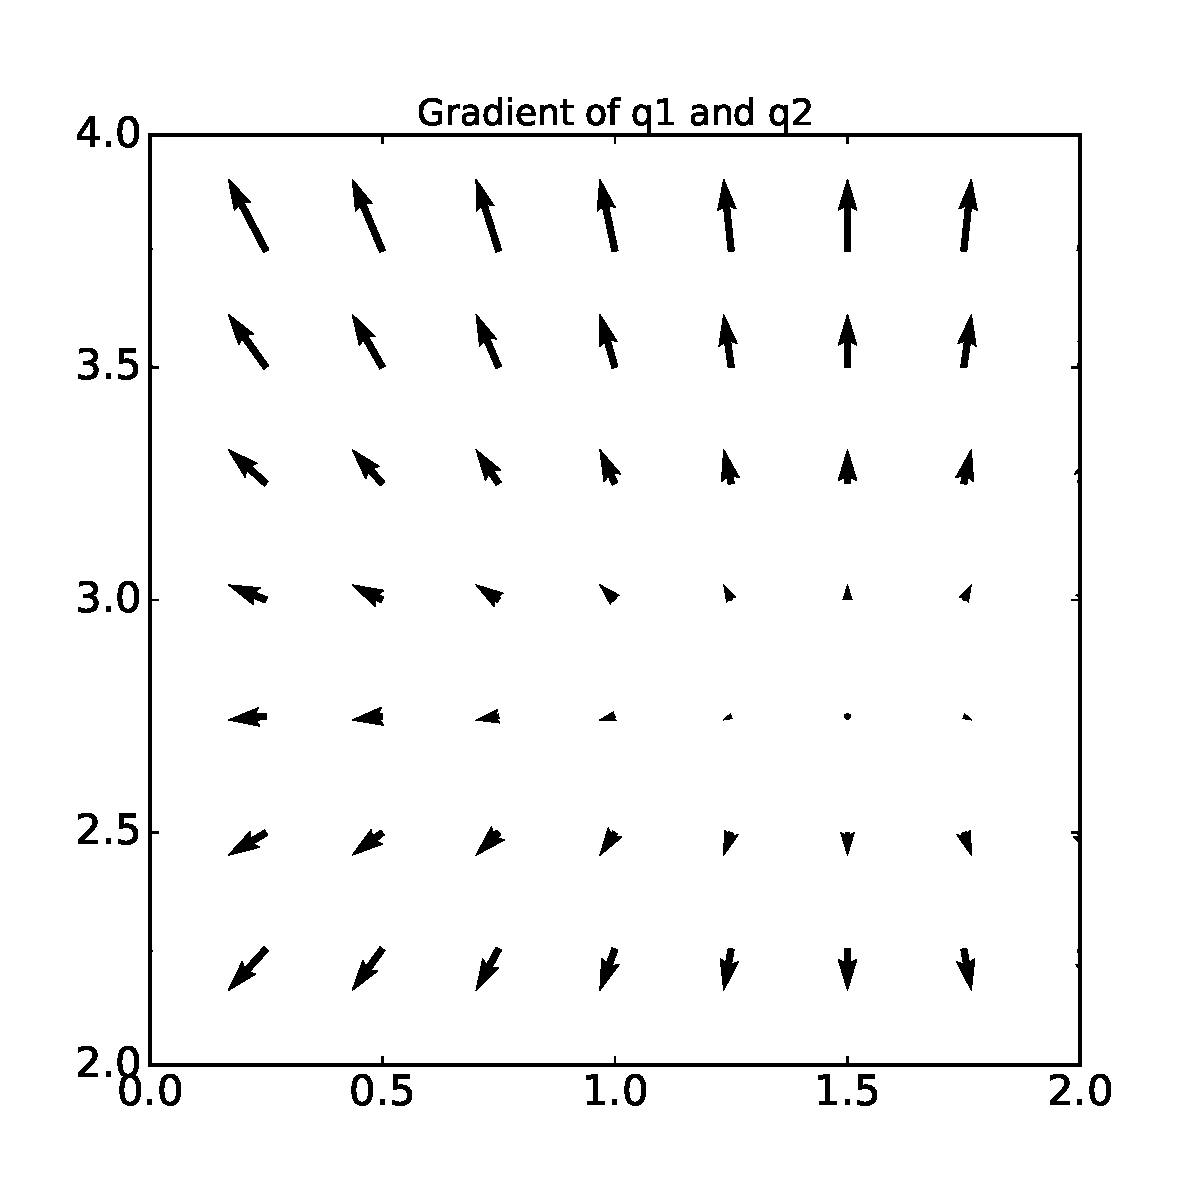
\includegraphics[width=\textwidth]{simple-linear-system/figures/gradient_2d_narrow_prior}
		\caption{Gradient with standard deviation $\sigma = 1$}
		\label{fig:linear_system.prior_influence.narrow}
	\end{subfigure}%
	\begin{subfigure}{.5\textwidth}
		\centering
		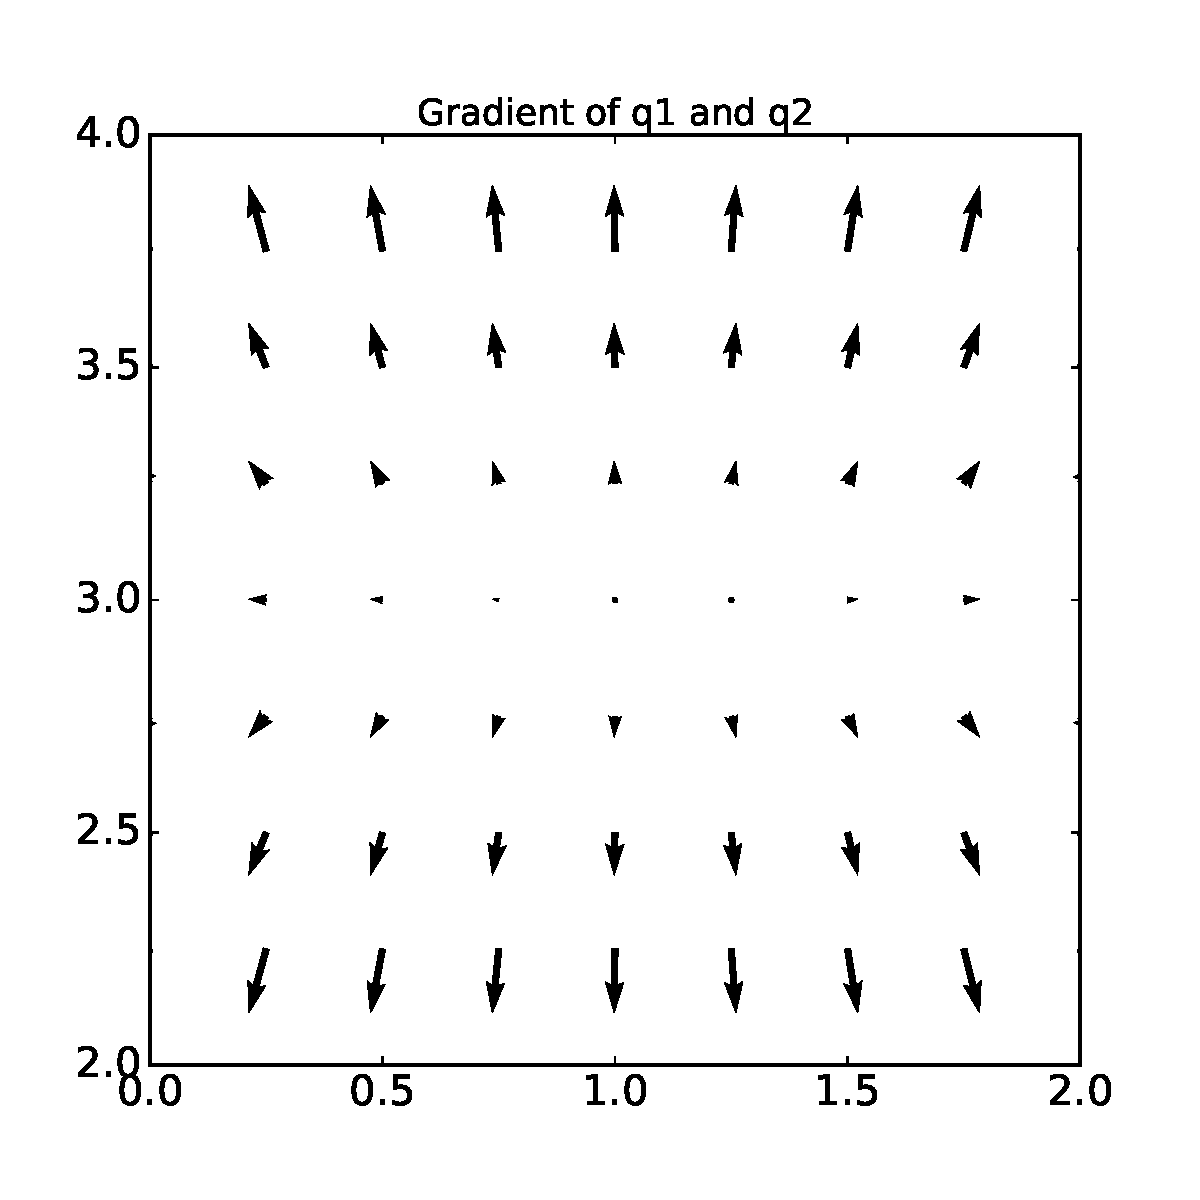
\includegraphics[width=\textwidth]{simple-linear-system/figures/gradient_2d_wide_prior}
		\caption{Gradient with standard deviation $\sigma = 5$}
		\label{fig:linear_system.prior_influence.wide}
	\end{subfigure}
	\caption{Normalized gradient of 2D misfit functionals with differently confined prior information. The means of the prior are for both parameters 2. It is obvious that decreasing the standard deviation for all parameters means that we increase the importance of the prior over the data, `pulling' the minimal gradient more towards the prior mean. Similar effects can be attained with increasing the magnitude of the data covariance matrix. Together, these matrices finely tune the minimum of the misfit function. Choosing well informed data and parameter covariace matrices is essential to meaningful \gls{HMC} sampling.}
	\label{fig:linear_system.prior_influence}
\end{figure}

\clearpage

\clearpage

\bibliography{sources.bib}
\printglossary
\printindex

\end{document}
